\chapter{Visualization}

\section{Making pictures using VTK}

VTK is a nice visualization toolkit tailored for scientific purposes. It builds on top of OpenGL and is available
for most platforms. One of the most useful features is the ability to define scientific data in e.g.\
grid form ("structured points") and to manipulate that data. Each grid point can contain various data forms:
scalars like temperature and pressure, but also vector data like velocity or fields.

There are several ways to visualize frameworks in RASPA using VTK:
\begin{itemize}
  \item{Ball and stick}\\
  RASPA will output vtk-files for all the molecules in the system as well as the framework itself.
  \item{Volume rendered surface area}\\
  RASPA will output a "structured point" grid of the adsorption energy. The structure is probed using Widom insertion
  at random positions and the result is averaged. The lowest and highest values are recorded and then scaled between
  0 and 2$^{16}$.
  \item{Volume rendered density plots of adsorbates}\\
  RASPA computes a 3D histogram of the positions of adsobates per component and for the total fluid.
  This type of plots are very useful to find out where and how the molecules adsorb.
\end{itemize}

\section{Ball and stick}

At the start of any run, RASPA outputs the current state in VTK files, located in `VTK/System[int]'. The files
are `FrameworkAtoms.vtk', `AdsorbateAtoms.vtk', `CationAtoms.vtk', and `Frame.vtk'. In 
`Example/Visualization/BallStickRASPA' the example for erionite is shown.
\begin{verbatim}
     SimulationType                   MC
     NumberOfCycles                   0

     Forcefield                       ExampleZeolitesForceField

     Framework 0
     FrameworkName ERI_mono
     UnitCells 1 1 1
\end{verbatim}

\begin{figure}[t]
  \centering
  \subfloat[]{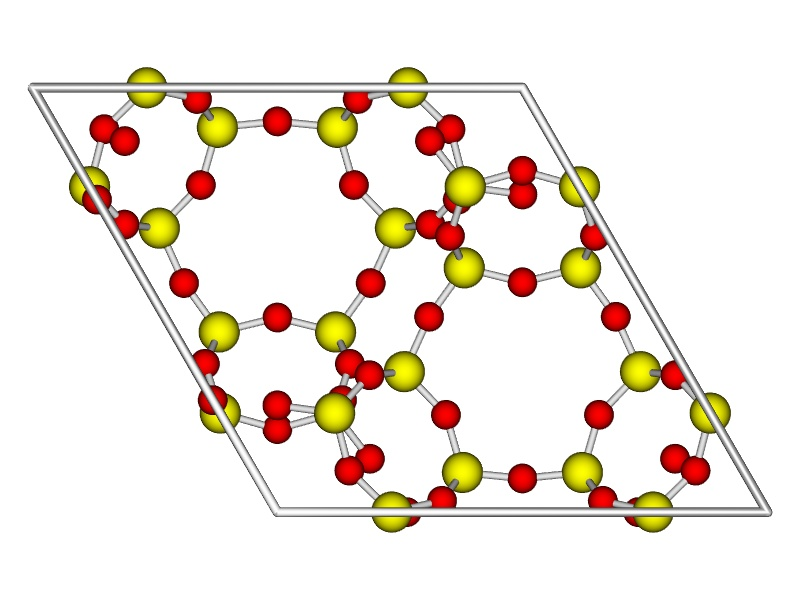
\includegraphics[width=7.5cm]{./Visualization/ERI_ball_stick_front.jpg}}
  \subfloat[]{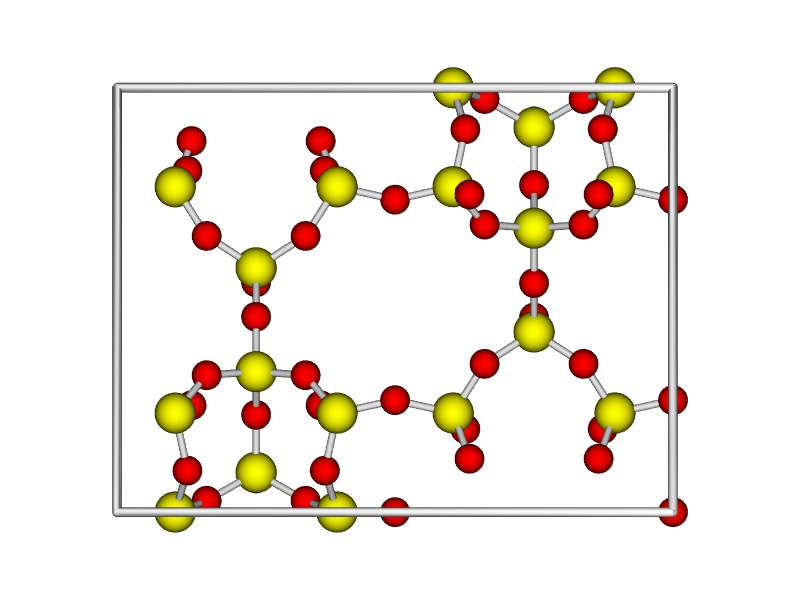
\includegraphics[width=7.5cm]{./Visualization/ERI_ball_stick_side.jpg}}
  \caption{Ball and stick picture of erionite (ERI): (a) front view, (b) side view. The erionite structure is
           monoclinic: $a=b=13.27$ \AA\ and $c=15.05$ \AA, $\alpha=\beta=90^\circ$ and $\gamma=120^\circ$.}
  \label{Fig: ERI ball-and-stick}
\end{figure}

After copying the vtk-files to `Examples/Visualization/ERI/VTK' one can run the VTK code. The VTK program
will produce a picture `Picture.jpg' and looks like Figure \ref{Fig: ERI ball-and-stick}.
The file `Frame.vtk' looks like:
\begin{verbatim}
     # vtk DataFile Version 1.0
     Frame
     ASCII

     DATASET POLYDATA
     POINTS 8 float
     50.000000 -0.000000 -0.000000
     150.000000 0.000000 0.000000
     100.000000 86.602540 0.000000
     0.000000 86.602540 0.000000
     50.000000 0.000000 113.413715
     150.000000 0.000000 113.413715
     100.000000 86.602540 113.413715
     0.000000 86.602540 113.413715
     LINES 6 36
     5 0 1 2 3 0
     5 4 5 6 7 4
     5 0 1 5 4 0
     5 2 3 7 6 2
     5 0 4 7 3 0
     5 1 2 6 5 1
\end{verbatim}
It contains 8 points: the corners of the frame, and 6 closed poly-lines that form the ribbons. Using the `vtkTubeFilter'
we can use these lines to turn them into bigger tubes and color the tubes white.
The coordinate system is chosen as $150\times150\times150$ to be compatible with structure grids (for the density and surface).
The information about the framework is listed in `FrameworkAtoms.vtk':
\begin{verbatim}
     # vtk DataFile Version 1.0
     Cube
     ASCII

     DATASET POLYDATA
     POINTS 108 float
     38.346000 20.221693 11.847197
     38.125000 36.762778 28.353429
     35.205000 30.250267 18.259608
     ....
     ....
     LINES 232 696
     2 0 2
     2 0 3
     2 0 13
     ....
     ....
     POINT_DATA 108
     SCALARS my_scalars float
     LOOKUP_TABLE default
     2.1
     2.1
     1.52
     ....
     ....
     VECTORS vectors float
     0.125 0 0
     0.125 0 0
     0.03125 0 0
     ....
     ....
\end{verbatim}
The first points are the 108 framework atoms, next the lines section describes the bonding between them.
The last two sections denote the size and color of the atoms (Note that the VECTORS section is a trick to
allow the VTK `glyphs', here spheres, to be scaled by the scalar data, but colored by the magnitude of the
VECTOR data. Hopefully this will be easier in future versions of VTK).

The VTK program is also interactive, one can zoom in and out (scroll button) and rotate (click on the canvas, closer
to the center rotates less then further away). In computer graphics, a sphere is not a sphere, but a collection
of polygons. More polygons means a smoother surface but less responsive in the interactive mode.
For final pictures, one should use many polygons and anti-aliasing, which really improve the quality of the
picture.

The VTK files are written in `src/movies.c' in the routine `void WriteVTK(int system)'. The top of this file also
defines the colors. This same color definition is also used in the VTK `main.c'.

\section{Framework surface}

The ball and stick pictures are useful, but still do not provide information about pore shape and connectivity.
A more suitable approach is to visualize the energy landscape for a certain probe atom.
For energy landscape pictures, we divide the unit cell
into e.g. $150\times150\times150$ voxels (volume-elements).
At millions of random positions in the unit cell
the free energy of a test-particle (usually a helium or methane unit atom) is calculated
and assigned to the appropriate voxel. To visualize this energy landscape
the three-dimensional dataset is volume rendered,
removing the parts that generate overlap (the structure itself) by making it
completely transparent.
Low energy values are rendered with medium transparency, allowing the inside of the pores/cages to
be viewed as voids. Higher energy values are rendered less and less
transparent until the energy approaches
a cutoff energy and is regarded as part of the zeolite wall. Also color is assigned according
to the energy value (green for the outside view of a cage).

To speed up computation of surface and density pictures it is advisable to use energy-grids. For the upcoming example
we need grids for CO$_2$-atoms and helium:

\begin{verbatim}
     SimulationType                   MakeGrid

     Forcefield                       ExampleZeolitesForceField

     Framework 0
     FrameworkName ERI_mono
     UnitCells 3 3 2
     ExternalTemperature 300.0

     NumberOfGrids 3
     GridTypes O_co2 C_co2 He
     SpacingVDWGrid 0.1
     SpacingCoulombGrid 0.1
\end{verbatim}
We need $3\times3\times2$ unit cells to obey the minimum-image convention.

Next we are going to generate the VTK `FrameworkatomsSurface.vtk' that contains data on the energy-grid for a chosen
probe atom. Here, we use helium.
An example input to generate the surface-grid is listed here (`Example/Visualization/ERI/SurfaceRASPA')
\begin{verbatim}
     SimulationType                   Visualization
     NumberOfCycles                   10000000000
     PrintEvery                       100000

     Forcefield                       ExampleZeolitesForceField
     ChargeMethod                     None

     Framework 0
     FrameworkName ERI_mono
     UnitCells 3 3 2
     ExternalTemperature 300.0

     NumberOfGrids 1
     GridTypes He
     SpacingVDWGrid 0.1
     SpacingCoulombGrid 0.1
     UseTabularGrid yes

     component 0 MoleculeName                     helium
                 MoleculeDefinition               ExampleDefinitions
                 IdealGasRosenbluthWeight         1.0
                 BlockPockets                     no
                 BlockPocketsFileName             ERI_mono
                 CreateNumberOfMolecules          0
\end{verbatim}

Even though the grid is generated for a single unit, in general one still needs $3\times3\times2$ unit cells because
the charge interaction is dependent on the amount of chosen unit cells.
The grid file `FrameworkSurface.vtk' is located in `VTK/System[int]'.

To visualize the pore-shape, copy the `FrameworkSurface.vtk' to `Examples/Visualization/ERI/VTK'. Do not copy the other VTK files
because they are generated for a $3\times3\times2$ grid, and we need the framework-atoms and frame- VTK files
for a $1\times1\times1$ structure.
Running the VTK-program now shows the surface inside the structure, as shown in
Figure \ref{Fig: ERI density}(a). If we compare Figure \ref{Fig: ERI density}(a) to Figure \ref{Fig: ERI ball-and-stick}
we see that we have visualized the pore structure itself. Also note, that small ``pockets'' have shown up that are not a
part of the main pore system. These pockets should be blocked (See next section).

The ERI-case by default offers a nice view inside the cage. This is not always the case. Using
\begin{verbatim}
     ShiftUnitCells 0.25 0 0 
\end{verbatim}
one can change the LTA case to a outside-cage-view to an inside-cage-view. (TODO, check whether grids takes this into account.)

\begin{figure}[t]
  \centering
  \subfloat[]{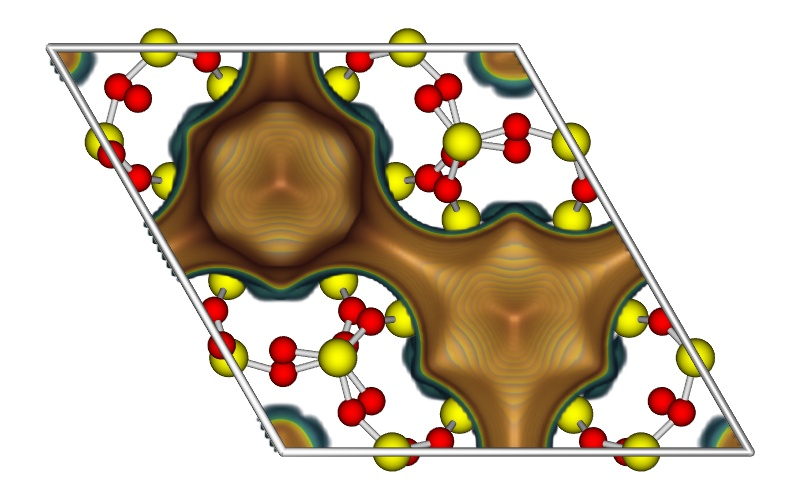
\includegraphics[width=7.5cm]{./Visualization/ERI_surface.jpg}}
  \subfloat[]{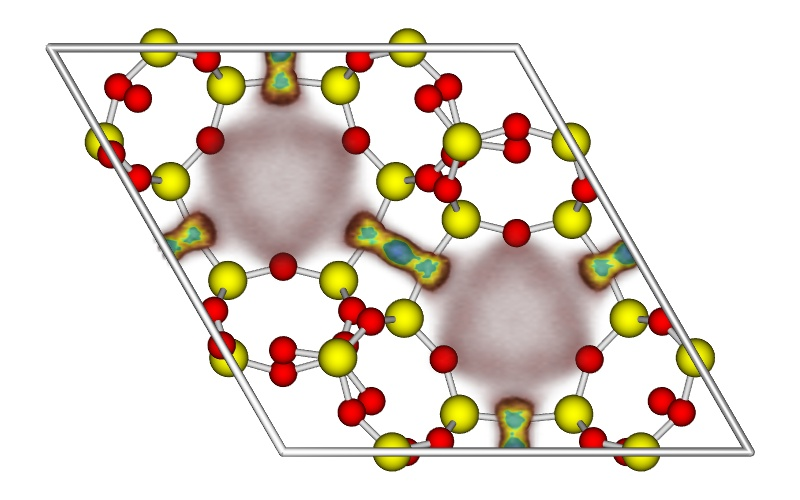
\includegraphics[width=7.5cm]{./Visualization/ERI_CO2_density.jpg}}
  \caption{Picture of ERI: (a) surface picture, (b) density picture (1 CO$_2$ at 300K).}
  \label{Fig: ERI density}
\end{figure}

The `FrameworkSurface.vtk' is a structured points VTK-file. It is rectangular grid of, in this case,
$150\times150\times150$ points (a total of 3375000 points). All these values are listed sequentially,
but one can convert between 1D and 3D by using 
\begin{equation}
\text{index}=x+y*\text{SIZEY}+z*\text{SIZEX}*\text{SIZEY}
\end{equation}
Note that the proper aspect ratios can be used. The VTK file looks like
\begin{verbatim}
     # vtk DataFile Version 1.0
     Free energy zeolite: ERI_mono (300.000000 K)
     ASCII
     DATASET STRUCTURED_POINTS
     DIMENSIONS 150 150 150
     ASPECT_RATIO 1.000000 0.577350 0.756091
     ORIGIN 0.0 0.0 0.0

     POINT_DATA 3375000
     SCALARS scalars unsigned_short
     LOOKUP_TABLE default
     0
     0
     ....
     ....
\end{verbatim}
The stored values are `unsigned short', so between 0 and 65536 ($2^{16}$). The value are always clipped to this region
using the minimum and maximum values of the simulation data.

\begin{figure}[t]
  \centering
  \hskip -0.5cm
  \subfloat[]{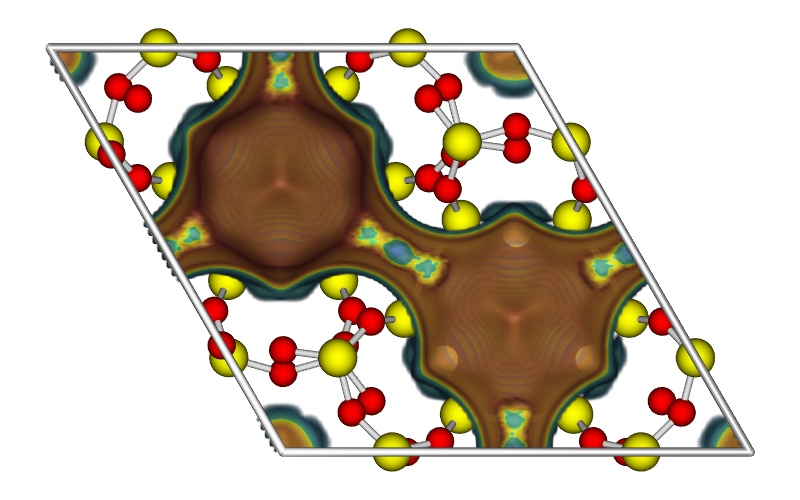
\includegraphics[width=7.5cm]{./Visualization/ERI_picture_all.jpg}}
  \hskip -0.5cm
  \subfloat[]{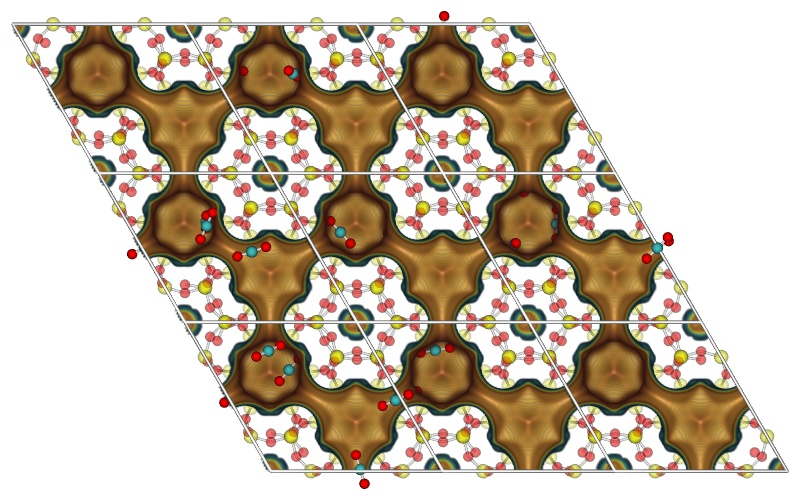
\includegraphics[width=9.75cm]{./Visualization/ERI_snapshot.jpg}}
  \caption{}
  \label{Fig: ERI picture all}
\end{figure}

\section{Density plots}

During a Monte Carlo simulation a 3-dimensional histogram of the positions
of all atoms of the molecules is collected (per component). The unit cell is divided into 150x150x150 "voxels".
During the simulation the molecules move around in the box, and every cycle data is collected
for the histogram. First a position is mapped back from the full simulation box (3x3x2 unit cells)
to the main unit cell, and for every atom the voxel corresponding to the mapped position is incremented.
At certain intervals the histogram is written to file so that it can be visualized using VTK.
The data is always normalized using the highest occurring voxel value. However, the overall brightness
is still influenced by the loading of the specific adsorbate in the mixture.

In VTK the data is "volume rendered", more dense regions are less transparent, less dense regions are
more transparent. In addition the color changes, less dense regions are grey, more dense are orange,
then yellow, and the highest is rendered light blue. The original framework is placed in the picture as
a ball-and-stick model, and every position can be related to the framework.
We can therefore e.g. decipher a molecular picture of why selectivity occurs.

An example input for RASPA is
\begin{verbatim}
     SimulationType                   MC
     NumberOfCycles                   100000000
     NumberOfInitializationCycles     100
     PrintEvery                       100
     PrintPropertiesEvery             10000

     Forcefield                       ExampleZeolitesForceField

     Framework 0
     FrameworkName ERI_mono
     UnitCells 3 3 2
     ExternalTemperature 300.0
     ComputeDensityProfile3DVTKGrid   yes
     WriteDensityProfile3DVTKGridEvery 10000
     DensityProfile3DVTKGridPoints 150 150 150

     NumberOfGrids 2
     GridTypes C_co2 O_co2
     SpacingVDWGrid 0.1
     SpacingCoulombGrid 0.1
     UseTabularGrid yes

     component 0 MoleculeName                     CO2
                 MoleculeDefinition               ExampleDefinitions
                 IdealGasRosenbluthWeight         1.0
                 TranslationProbability           1.0
                 RegrowProbability                1.0
                 SwapProbability                  0.0
                 CreateNumberOfMolecules          1
\end{verbatim}

Copy the `VTK/System[int]/DensityProfile\_methane.vtk' to `Examples/Visualization/ERI/VTK' as `Density.vtk',
rename the surface VTK-file,
and run the vtk-code. It will now produce a picture like Figure \ref{Fig: ERI density}(b).
If you did not rename the file (or rename it again to `FrameworkatomsSurface.vtk'), a picture with the frameworks atoms,
the pore surface and the density of CO$_2$ is produced. It is now easy to show that CO$_2$ preferentially adsorbs
in the 8-ring windows separating the erionite cages (in contrast to an alkane which prefers the cages).

Of course, one is not restricted to a unit cell and it is possible to make pictures of bigger volumes.
The first way is to use $3\times3\times2$ unit cells, and use the file `Movies/System[int]/Framework\_initial.cssr'.
Copy this file as `structure\_name\_3x3x2.cssr' and from then on use $1\times1\times1$ using this new enlarged unit cell.
The second method is to use $3\times3\times2$ unit cell but copy the surface and density in the $x$, $y$, $z$ directions
in the picture. You have to edit the `main.c' file of the VTK directory and recompile. The relevant settings are:
\begin{verbatim}
     // the resolution of spheres and tubes, the higher the more smooth
     // use 10, but 50 for the final picture
     const int Resolution=10;

     // anti-aliasing, use 1, but 16 for final picture
     const int AA=1;

     // control the transparancy of framework, adsorbates, and cations
     const double FrameworkOpacity=1.0;
     const double AdsorbateOpacity=1.0;
     const double CationOpacity=1.0;

     // zoom in or out by increasing/decreasing the zoom-factor
     const double ZoomFactor=2.0;

     // scale the size of the atoms and bonds
     const double ScaleFactor=1.0;

     // control the view-point of the oject (input in degrees)
     const double Azimuth=0.0;
     const double Elevation=0.0;
     const double Roll=0.0;

     // the size of the image in pixels
     const int ImageSizeX=800;
     const int ImageSizeY=500;

     // the number of duplicates in x,y,z (same as the number of unit cells)
     const int NrDuplicatesX=3;
     const int NrDuplicatesY=3;
     const int NrDuplicatesZ=2;

     // the lengths of the edge-vectors
     const double A=13.27;
     const double B=13.27;
     const double C=15.05;

     // the angles of the unit cell
     const double AlphaAngle=90*M_PI/180.0;
     const double BetaAngle=90*M_PI/180.0;
     const double GammaAngle=120*M_PI/180.0;
\end{verbatim}
This can then be used to make a `snapshot' of molecules. For the $3\times3\times2$ structure we need the file
`VTK/System[int]/AdsorbateAtoms.vtk' from a simulation. This file is generated at the start of a simulation. 
After a sufficiently long run to equilibrate the molecules, one
could copy the `Restart' to `RestartInitial', put the amount of created molecules at zero and restart from the
restart-files using zero cycles to generate the new `AdsorbateAtoms.vtk' file.
The picture of a snapshot of 64 CO$_2$ in the $3\times3\times2$ ERI-structure is shown in
Figure \ref{Fig: ERI picture all}(b). Note the many CO$_2$ molecules that occupy the barrier. Conclusions
are hard to draw based on snapshots. The `density'-plots give average information and therefore the same for
each unit cell (because each unit cell is the same [using a rigid structure]). The density plots are based on
atoms, and one can clearly see the orientation of CO$_2$ on the barrier. The 3 `blobs' corresponds to the oxygen, carbon,
and oxygen of CO$_2$.

\begin{figure}[t]
  \centering
  \subfloat[]{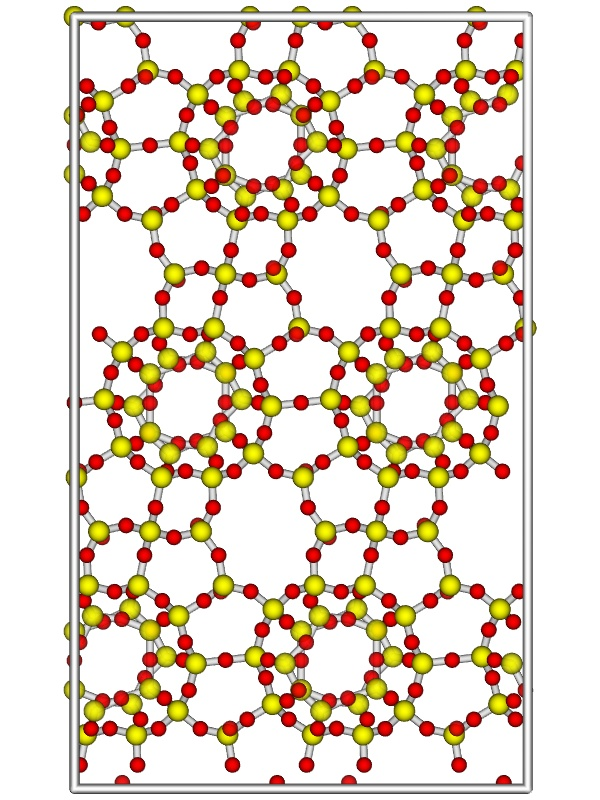
\includegraphics[width=5.0cm]{./Visualization/DDR_picture_1.jpg}}
  \subfloat[]{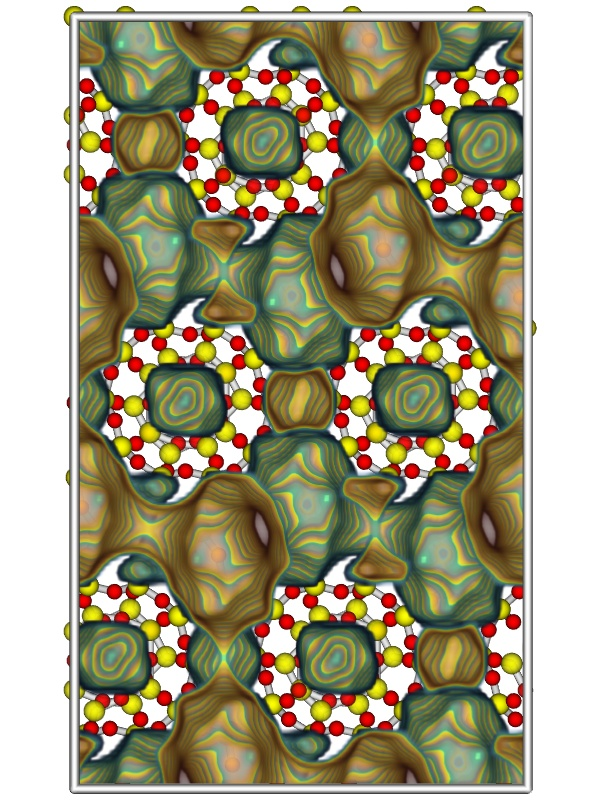
\includegraphics[width=5.0cm]{./Visualization/DDR_picture_2.jpg}}
  \subfloat[]{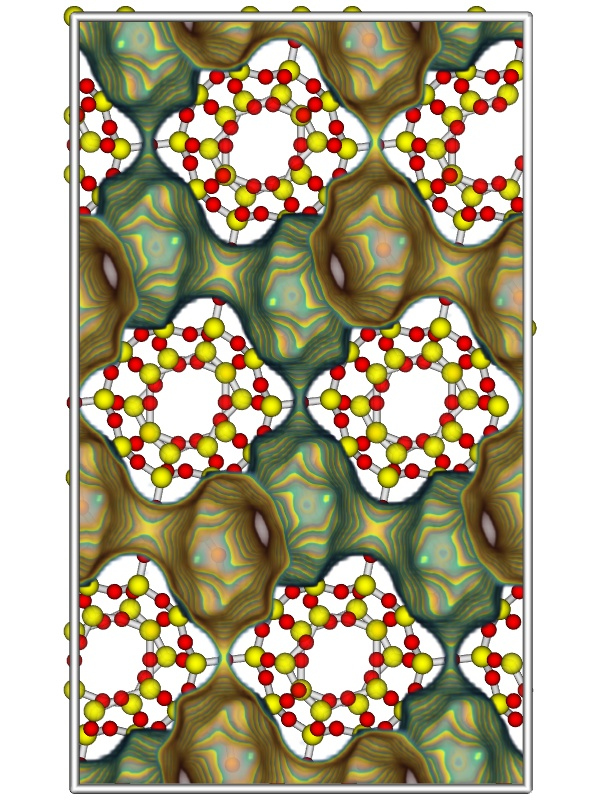
\includegraphics[width=5.0cm]{./Visualization/DDR_picture_3.jpg}}
  \caption{Blocking pockets in DDR. The DDR structure is converted to a orthorhombic unit cell of
   $a=24.006,b=13.86$, and $c=40.892$ \AA. In (a) we show the ball-and-stick structure, in (b) the structure
   and the pore surface probed with helium, and (c) the structure with proper blocking of the small disconnected pockets.}
  \label{Fig: DDR blocking}
\end{figure}

\section{Determining blocking pockets}

Some structures have inaccessible parts, i.e. areas that are not reachable from the main pore system. Examples
are the sodalite cages in FAU- and LTA-type zeolites. The surface pictures allow us to visualize these pockets,
locate the position, and construct a `blocking-file'.

The unit cell of the DDR structure has edge lengths of a=24.006 Angstrom, b=13.86 Angstrom, 40.892 Angstrom 
with cell angles of 90 degrees. The atomic structure is shown in Figure \ref{Fig: DDR blocking}(a). It is difficult to envision 
the details of the pore structure from this picture. One can obtain more insight from energy-landscapes.
In Figure \ref{Fig: DDR blocking}(b) we show the same structure with the energy landscape a helium atom would feel. In practice, 
the simulation cell is divided into 150x150x150 bins and during a Monte-Carlo simulation one keeps track of 
the average energy a molecule feels inside that bin. Here we volume-rendered the resulting energy grid 
making very high energies transparent, i.e. the part that overlaps with the framework, as well as very 
favorable energies, i.e. the positions inside the cage. The resulting surface layer can be viewed as the 
"wall" of the pores. Alternatively, one can make a isocontour (a surface representing a constant, 
high value of the energy). In Figure \ref{Fig: DDR blocking}(b) the main pore structure is apparent, 
but also some disconnect pockets show up. It is 
very important to artificially block these pockets for Monte-Carlo simulations. Also, in 
Molecular Dynamic simulations, initial positions should be chosen in the main channel system. The blocking 
procedure can be a simple distance-check from the center of the small pockets and a rejection of all 
Monte-Carlo trial moves that would place a molecule inside a certain radius. This radius should not be 
chosen to small or too big, because otherwise one would block not enough, or block parts of the 
main channel system. In Figure \ref{Fig: DDR blocking}(c) we show the structure with the appropriate blocking centers and radii; 
all small pockets have disappeared but the main channel system is unchanged.

The blocking procedure is dependent on the type of probe atom. Helium is a good procedure to find small pockets 
and therefore to obtain the proper unit cell pore volume. This accessible pore volume is in simulation 
usually obtained via a helium-probe procedure. Helium can also be used to find pockets that 
could be occupied by other small molecule like CO2, N2, H2, methane, etc.
The adsorption results can be dramatically different with or without blocking. Whether the selectivity of 
mixtures changes to higher or lower depends on the match of the molecule with the small pockets. 
The small pockets are very favorable for the small molecules because they tend to have a very surface high 
curvature, i.e.. a very favorable interaction energy). 

\section{Making movies}

\subsection{Using VMD}

\subsection{Combining pictures into a movie}

Using ``ffmpeg'', from png-files to a mov-file with h264-encoding
\begin{verbatim}
ffmpeg -i %03d.png -s:v 1280x720  -acodec aac -ac 2 -strict experimental -ab 160k 
-vcodec libx264 -preset slow -profile:v baseline -level 30 -maxrate 10000000 
-bufsize 10000000 -b 1200k -f mp4 -threads 0  -crf 23 -pix_fmt yuv420p -r 30 Movie.mov 
\end{verbatim}
or using ``mencoder'' with settings 
\begin{footnotesize}
\begin{verbatim}
export opt="vbitrate=1280000:mbd=2:keyint=132:vqblur=1.0:cmp=2:subcmp=2:dia=2:mv0:last_pred=3"
mencoder -ovc lavc -lavcopts vcodec=msmpeg4v2:vpass=1:$opt -mf type=jpg:fps=25 -nosound -o /dev/null mf://\*.jpg
mencoder -ovc lavc -lavcopts vcodec=msmpeg4v2:vpass=2:$opt -mf type=jpg:fps=25 -nosound -o output.avi mf://\*.jpg
\end{verbatim}
\end{footnotesize}

